%% Chapter 25: Neural Networks in the Loop
%% IEEE-Formatted Control Systems Textbook
%% Self-contained chapter with complete derivations and practical experiments

\chapter{Neural Networks in the Loop}
\label{ch:neural_networks}

\begin{quote}
\textit{``A computer would deserve to be called intelligent if it could deceive a human into believing that it was human.''} --- Alan Turing, 1950
\end{quote}

\section{Historical Motivation: From Biological Neurons to Learning Machines}

The marriage of neural networks and control systems represents one of the most significant developments in modern engineering. This union brings together two distinct intellectual traditions: the mathematical rigor of control theory and the adaptive, data-driven philosophy of machine learning. Understanding this history illuminates why neural networks have become indispensable tools for controlling complex systems that resist traditional modeling approaches.

\subsection{McCulloch and Pitts (1943): The Computational Neuron}

In 1943, neurophysiologist Warren McCulloch and mathematician Walter Pitts published ``A Logical Calculus of the Ideas Immanent in Nervous Activity,'' a paper that would lay the foundation for both artificial intelligence and neural computation. Working at the University of Illinois, they asked a deceptively simple question: could the behavior of biological neurons be described mathematically?

Their key insight was that neurons could be modeled as binary threshold units. A biological neuron receives inputs from other neurons through synaptic connections, integrates these signals, and ``fires'' (produces an output) if the integrated signal exceeds a threshold. McCulloch and Pitts formalized this as:
\begin{equation}
y = \begin{cases} 1 & \text{if } \sum_{i} w_i x_i \geq \theta \\ 0 & \text{otherwise} \end{cases}
\label{eq:mcculloch_pitts}
\end{equation}
where $x_i$ are binary inputs, $w_i$ are synaptic weights, and $\theta$ is the threshold.

The profound implication was that networks of such simple units could, in principle, compute any logical function. This was the birth of the computational theory of mind and the first mathematical model of neural computation. However, McCulloch and Pitts did not address how such networks might \textit{learn}---the weights were assumed to be fixed.

\subsection{Rosenblatt (1958): The Perceptron and Learning}

Frank Rosenblatt, a psychologist at Cornell, took the crucial next step. In 1958, he introduced the \textbf{Perceptron}, a device that could \textit{learn} to classify patterns by adjusting its weights based on errors. The Perceptron learning rule was elegant:
\begin{equation}
w_i^{\text{new}} = w_i^{\text{old}} + \eta (y_{\text{desired}} - y_{\text{actual}}) x_i,
\label{eq:perceptron_rule}
\end{equation}
where $\eta$ is a learning rate. If the output is correct, no change occurs. If the output is wrong, weights are adjusted to reduce the error.

Rosenblatt demonstrated the Perceptron on the Mark I Perceptron machine at Cornell, which used photocells to ``see'' images and could learn to distinguish simple shapes. The New York Times reported in 1958 that the Navy had unveiled ``an electronic computer that will be able to walk, talk, see, write, reproduce itself, and be conscious of its existence.'' This was, of course, hyperbole, but the excitement was palpable.

The Perceptron Convergence Theorem proved that if a linear separation of the data exists, the Perceptron algorithm will find it in finite time. This was a remarkable guarantee---but it contained the seeds of the coming crisis.

\subsection{Minsky and Papert (1969): The First AI Winter}

In 1969, Marvin Minsky and Seymour Papert published \textit{Perceptrons}, a rigorous mathematical analysis of what single-layer perceptrons could and could not compute. Their most devastating result: a perceptron cannot learn the XOR function. More generally, perceptrons could only represent linearly separable functions.

\begin{figure}[htbp]
\centering
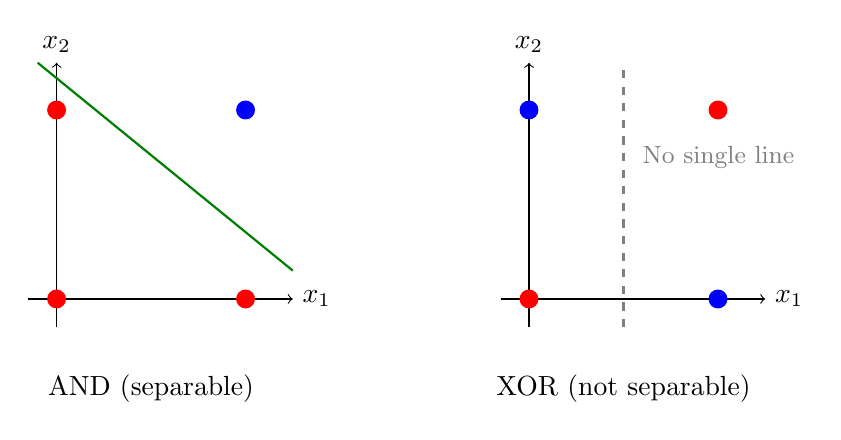
\begin{tikzpicture}[scale=1.2]
% AND function (linearly separable)
\begin{scope}[shift={(0,0)}]
\draw[->] (-0.3,0) -- (2.5,0) node[right] {$x_1$};
\draw[->] (0,-0.3) -- (0,2.5) node[above] {$x_2$};
\fill[red] (0,0) circle (0.1);
\fill[red] (0,2) circle (0.1);
\fill[red] (2,0) circle (0.1);
\fill[blue] (2,2) circle (0.1);
\draw[thick, green!50!black] (-0.2,2.5) -- (2.5,0.3);
\node[below] at (1,-0.7) {AND (separable)};
\end{scope}

% XOR function (not linearly separable)
\begin{scope}[shift={(5,0)}]
\draw[->] (-0.3,0) -- (2.5,0) node[right] {$x_1$};
\draw[->] (0,-0.3) -- (0,2.5) node[above] {$x_2$};
\fill[red] (0,0) circle (0.1);
\fill[blue] (0,2) circle (0.1);
\fill[blue] (2,0) circle (0.1);
\fill[red] (2,2) circle (0.1);
\draw[thick, dashed, gray] (1,-0.3) -- (1,2.5);
\node[right, gray, font=\small] at (1.1,1.5) {No single line};
\node[below] at (1,-0.7) {XOR (not separable)};
\end{scope}
\end{tikzpicture}
\caption{The XOR problem illustrated. AND can be separated by a single line; XOR cannot. Blue dots represent output 1, red dots represent output 0.}
\label{fig:xor_problem}
\end{figure}

While Minsky and Papert acknowledged that multi-layer networks could overcome this limitation, they expressed skepticism that effective training algorithms would be found. Funding for neural network research collapsed, initiating what historians call the first ``AI Winter'' (roughly 1969--1982). Many researchers abandoned the field entirely.

\begin{historicalbox}[The Perceptron Media Frenzy]
The original excitement around the Perceptron in 1958 generated extraordinary media coverage. The New York Times reported that the Navy expected the Perceptron to ``walk, talk, see, write, reproduce itself and be conscious of its existence.'' Frank Rosenblatt himself was more measured, but the disconnect between public expectations and technical reality would become a recurring theme in AI history. When Minsky and Papert published their critique eleven years later, the resulting backlash was equally dramatic---neural network funding virtually disappeared overnight, and researchers who continued in the field faced professional marginalization. This boom-bust cycle has repeated several times in AI history, teaching the important lesson that managing expectations is as crucial as technical progress.
\end{historicalbox}

\subsection{Werbos (1974) and Rumelhart et al. (1986): Backpropagation}

The key to training multi-layer networks had actually been discovered in 1974 by Paul Werbos in his Harvard PhD thesis, ``Beyond Regression: New Tools for Prediction and Analysis in the Behavioral Sciences.'' Werbos developed \textbf{backpropagation}---an algorithm for computing gradients through multi-layer networks using the chain rule of calculus.

However, Werbos's work was largely ignored by the AI community. It was not until 1986, when David Rumelhart, Geoffrey Hinton, and Ronald Williams published ``Learning Representations by Back-propagating Errors'' in \textit{Nature}, that backpropagation gained widespread attention. The algorithm enabled training of \textbf{multi-layer perceptrons} (MLPs) that could learn non-linear functions, including XOR.

The key insight was expressing learning as an optimization problem:
\begin{equation}
\min_{\mathbf{w}} \mathcal{L}(\mathbf{w}) = \min_{\mathbf{w}} \frac{1}{N}\sum_{i=1}^{N} \|y_i - f(\mathbf{x}_i; \mathbf{w})\|^2,
\label{eq:loss_function}
\end{equation}
where $f(\mathbf{x}; \mathbf{w})$ is the neural network with weights $\mathbf{w}$. Backpropagation computes $\partial \mathcal{L}/\partial w_j$ efficiently, enabling gradient descent optimization.

\subsection{Narendra and Parthasarathy (1990): Neural Networks Meet Control}

The pivotal moment for neural networks in control came with Kumpati Narendra and Kannan Parthasarathy's 1990 paper, ``Identification and Control of Dynamical Systems Using Neural Networks,'' published in \textit{IEEE Transactions on Neural Networks}. This landmark work systematically explored how neural networks could serve in three fundamental capacities. First, as \textbf{system identifiers}, neural networks could learn the dynamics $\hat{f}$ such that $\mathbf{x}[k+1] \approx \hat{f}(\mathbf{x}[k], \mathbf{u}[k])$, enabling prediction of system behavior without explicit analytical models. Second, as \textbf{controllers}, they could compute control actions $\mathbf{u} = g(\mathbf{x})$ to achieve desired behavior through learned mappings from states to inputs. Third, as \textbf{inverse models}, neural networks could learn the inverse dynamics for feedforward control, computing the inputs required to produce desired outputs.

Narendra and Parthasarathy demonstrated that neural networks could approximate nonlinear plant dynamics and serve as adaptive controllers. Their framework established the theoretical foundation for neural network control that remains influential today.

\begin{figure}[htbp]
\centering
\begin{tikzpicture}[node distance=2cm, scale=0.9, transform shape]
% Styles
\tikzset{
    block/.style={draw, rectangle, minimum height=1.5cm, minimum width=2cm, align=center},
    sum/.style={draw, circle, inner sep=0.1cm},
    arrow/.style={->, thick}
}

% Direct inverse control
\node[block, fill=blue!20] (nn) {Neural\\Network\\Controller};
\node[block, fill=gray!20, right=2cm of nn] (plant) {Plant};
\node[left=1.5cm of nn] (ref) {$r$};
\node[right=1.5cm of plant] (output) {$y$};

\draw[arrow] (ref) -- (nn);
\draw[arrow] (nn) -- node[above] {$u$} (plant);
\draw[arrow] (plant) -- (output);

% Feedback path
\draw[arrow] (plant.east) -- ++(0.5,0) -- ++(0,-1.5) -| (nn.south);

\node[below=0.3cm of plant] {(a) NN as Controller};

% Model reference
\begin{scope}[shift={(0,-5)}]
\node[block, fill=green!20] (model) {Reference\\Model};
\node[block, fill=blue!20, below=1cm of model] (nn2) {Neural\\Network};
\node[block, fill=gray!20, right=2cm of nn2] (plant2) {Unknown\\Plant};
\node[sum, left=1.5cm of model] (sum1) {};
\node[sum, right=3.5cm of model] (sum2) {};
\node[left=0.8cm of sum1] (ref2) {$r$};
\node[right=0.8cm of sum2] (error) {$e$};

\draw[arrow] (ref2) -- (sum1);
\draw[arrow] (sum1) -- (model);
\draw[arrow] (sum1) |- (nn2);
\draw[arrow] (nn2) -- node[above] {$u$} (plant2);
\draw[arrow] (model) -- node[above] {$y_m$} (sum2);
\draw[arrow] (plant2) -- ++(1,0) |- (sum2);
\draw[arrow] (sum2) -- (error);
\draw[arrow] (plant2.east) -- ++(0.5,0) -- ++(0,-1) -| (nn2.south);
\node[right] at (plant2.east) {$y_p$};

\node[below=0.3cm of plant2] {(b) Model Reference Adaptive Control};
\end{scope}
\end{tikzpicture}
\caption{Neural network control architectures from Narendra and Parthasarathy (1990). (a) Direct neural network controller. (b) Model reference adaptive control with neural network.}
\label{fig:narendra_architectures}
\end{figure}

\subsection{The Second AI Winter and Deep Learning Revolution}

Despite the promise shown in the early 1990s, neural networks faced practical limitations: training was slow, networks were prone to overfitting, and results were often inconsistent. Support Vector Machines and other kernel methods, with their convex optimization guarantees, became the preferred tools. A second AI Winter descended on neural network research (roughly 1995--2010).

The deep learning revolution began in 2006 when Geoffrey Hinton and colleagues demonstrated that \textbf{deep neural networks} (with many layers) could be trained effectively using layer-wise pre-training. The breakthrough came in 2012 when Alex Krizhevsky's ``AlexNet'' won the ImageNet competition by a large margin using a deep convolutional neural network trained on GPUs.

Several enabling factors converged to make this revolution possible. Massive datasets such as ImageNet provided millions of labeled images for training. GPU computing enabled parallel processing that accelerated training by 10--100$\times$ compared to CPU-only approaches. Algorithmic improvements including ReLU activations, dropout, and batch normalization addressed the vanishing gradient problem and improved generalization. Finally, software frameworks like TensorFlow and PyTorch made implementation accessible to researchers and practitioners alike.

\subsection{Why Neural Networks for Control?}

Neural networks offer several compelling advantages for control applications. The property of \textbf{universal function approximation} guarantees that, given enough neurons, a neural network can approximate any continuous function to arbitrary accuracy (Cybenko, 1989; Hornik, 1991), enabling representation of complex nonlinear dynamics that defy analytical modeling. The ability to \textbf{learn from data} rather than deriving models from first principles proves invaluable when physics-based models are unavailable or too complex. Neural networks naturally \textbf{handle high-dimensional inputs} like images, enabling end-to-end learning from raw sensor data to control actions without manual feature engineering. Additionally, their \textbf{adaptability} through online learning allows neural network controllers to adjust to changing plant dynamics or operating conditions in real time.

However, neural networks also present significant challenges for control. Unlike linear controllers designed via pole placement, neural network controllers provide \textbf{no inherent stability guarantees}, making safety-critical deployment difficult. The ``black box'' nature creates \textbf{interpretability} challenges, making it difficult to understand why a controller takes certain actions or to predict behavior in novel situations. Finally, \textbf{data requirements} for training can be substantial, and collecting such data from physical systems may be expensive, time-consuming, or dangerous.

These challenges motivate the hybrid approaches discussed later in this chapter.


\section{Modern Applications of Neural Networks in Control}

Neural networks have moved from academic curiosity to production systems controlling vehicles, robots, and industrial processes. This section surveys current applications.

\subsection{End-to-End Autonomous Driving}

The most visible application of neural networks in control is autonomous driving. Traditional approaches decompose driving into perception (detecting lanes, vehicles, pedestrians), planning (determining a trajectory), and control (executing the trajectory). Neural networks now appear in all three stages.

In \textbf{end-to-end learning}, pioneered by NVIDIA's DAVE-2 system (2016), a single neural network maps directly from camera images to steering commands. The network is trained on human driving data using behavioral cloning:
\begin{equation}
\min_{\theta} \sum_{i} \|u_{\text{human},i} - f_{\theta}(\text{image}_i)\|^2.
\end{equation}

Companies like Tesla, Waymo, and Comma.ai deploy neural network-based systems processing multiple camera feeds, radar, and lidar to generate control commands in real-time. These systems must handle edge cases, adverse weather, and unpredictable human behavior.

\subsection{Neural Network Controllers for Drones}

Quadrotor drones present challenging control problems: they are underactuated (4 inputs controlling 6 degrees of freedom), nonlinear, and must operate in turbulent environments. Neural networks have enabled capabilities beyond traditional controllers, including agile flight through reinforcement learning that achieves acrobatic maneuvers difficult to hand-design, recovery from failures where networks learn to fly with damaged rotors, and visual navigation where end-to-end networks fly through forests using only onboard cameras.

The key advantage is that neural networks can learn complex mappings from sensor inputs to motor commands that account for aerodynamic effects, motor saturation, and sensor noise in ways that analytical models cannot.

\subsection{Learned Dynamics Models for MPC}

Model Predictive Control (Chapter~\ref{ch:mpc}) requires a dynamics model to predict future states. When analytical models are unavailable or inaccurate, neural networks can learn the dynamics:
\begin{equation}
\mathbf{x}[k+1] = f_{\theta}(\mathbf{x}[k], \mathbf{u}[k]).
\end{equation}

This learned model is then used within the MPC optimization:
\begin{equation}
\min_{\mathbf{u}[k], \ldots, \mathbf{u}[k+N-1]} \sum_{j=0}^{N-1} \ell(\hat{\mathbf{x}}[k+j], \mathbf{u}[k+j]) + V_f(\hat{\mathbf{x}}[k+N])
\end{equation}
where $\hat{\mathbf{x}}$ are states predicted by the neural network model.

Applications include robot manipulation, chemical process control, and building energy management, where first-principles models are either unavailable or too computationally expensive for real-time MPC.

\subsection{Industrial Soft Sensors}

In chemical and manufacturing processes, key quality variables (product composition, viscosity, molecular weight) are often difficult or expensive to measure directly. \textbf{Soft sensors} use neural networks to estimate these variables from readily available measurements (temperature, pressure, flow rates):
\begin{equation}
\hat{y}_{\text{quality}} = f_{\theta}(T, P, F, \ldots).
\end{equation}

These neural network estimators enable closed-loop control of quality variables that would otherwise require delayed laboratory analysis. Applications include polymer production, petroleum refining, and semiconductor manufacturing.


\section{Mathematical Foundation: Neural Networks for Dynamics and Control}

We now develop the mathematical framework for using neural networks in control systems. This section provides complete derivations suitable for implementation.

\subsection{The Artificial Neuron}

The fundamental building block is the artificial neuron, which computes a weighted sum of inputs, adds a bias, and applies a nonlinear activation function:
\begin{equation}
y = \sigma\left(\sum_{i=1}^{n} w_i x_i + b\right) = \sigma(\mathbf{w}^T\mathbf{x} + b),
\label{eq:neuron}
\end{equation}
where $\mathbf{x} = [x_1, \ldots, x_n]^T \in \mathbb{R}^n$ is the input vector, $\mathbf{w} = [w_1, \ldots, w_n]^T \in \mathbb{R}^n$ is the weight vector, $b \in \mathbb{R}$ is the bias term, $\sigma: \mathbb{R} \to \mathbb{R}$ is the activation function, and $y \in \mathbb{R}$ is the scalar output.

\begin{figure}[htbp]
\centering
\begin{tikzpicture}[scale=1.0]
% Input nodes
\foreach \i in {1,2,3} {
    \node[circle, draw, minimum size=0.8cm] (x\i) at (0, 2-\i) {$x_{\i}$};
}
\node at (0, -1.5) {$\vdots$};
\node[circle, draw, minimum size=0.8cm] (xn) at (0, -2.5) {$x_n$};

% Summation node
\node[circle, draw, minimum size=1.2cm, fill=blue!20] (sum) at (3, -0.25) {$\Sigma$};

% Activation node
\node[circle, draw, minimum size=1.2cm, fill=green!20] (sigma) at (5.5, -0.25) {$\sigma$};

% Output
\node[circle, draw, minimum size=0.8cm] (y) at (8, -0.25) {$y$};

% Bias node
\node[circle, draw, minimum size=0.8cm, fill=gray!20] (b) at (3, -2.5) {$b$};

% Connections
\foreach \i in {1,2,3} {
    \draw[->, thick] (x\i) -- (sum) node[midway, above, sloped, font=\small] {$w_{\i}$};
}
\draw[->, thick] (xn) -- (sum) node[midway, above, sloped, font=\small] {$w_n$};
\draw[->, thick] (b) -- (sum);
\draw[->, thick] (sum) -- (sigma) node[midway, above, font=\small] {$z$};
\draw[->, thick] (sigma) -- (y);

% Labels
\node[below=0.3cm of sum, font=\small] {Weighted sum};
\node[below=0.3cm of sigma, font=\small] {Activation};
\end{tikzpicture}
\caption{Structure of an artificial neuron. Inputs $x_i$ are multiplied by weights $w_i$, summed with bias $b$, and passed through activation function $\sigma$.}
\label{fig:neuron}
\end{figure}

\subsection{Activation Functions}

The choice of activation function $\sigma$ determines the neuron's nonlinear behavior. Common choices include:

\textbf{Sigmoid:}
\begin{equation}
\sigma(z) = \frac{1}{1 + e^{-z}}, \quad \sigma'(z) = \sigma(z)(1 - \sigma(z))
\end{equation}
Output range: $(0, 1)$. Historically popular but suffers from vanishing gradients.

\textbf{Hyperbolic Tangent (tanh):}
\begin{equation}
\sigma(z) = \tanh(z) = \frac{e^z - e^{-z}}{e^z + e^{-z}}, \quad \sigma'(z) = 1 - \tanh^2(z)
\end{equation}
Output range: $(-1, 1)$. Zero-centered, but also suffers from vanishing gradients.

\textbf{Rectified Linear Unit (ReLU):}
\begin{equation}
\sigma(z) = \max(0, z), \quad \sigma'(z) = \begin{cases} 1 & z > 0 \\ 0 & z \leq 0 \end{cases}
\end{equation}
Output range: $[0, \infty)$. Computationally efficient, addresses vanishing gradients, but can cause ``dead neurons'' when $z < 0$.

\textbf{Leaky ReLU:}
\begin{equation}
\sigma(z) = \begin{cases} z & z > 0 \\ \alpha z & z \leq 0 \end{cases}
\end{equation}
where $\alpha \approx 0.01$ prevents dead neurons.

\begin{figure}[htbp]
\centering
\begin{tikzpicture}[scale=0.8]
% Sigmoid
\begin{scope}[shift={(0,0)}]
\draw[->] (-3,0) -- (3,0) node[right] {$z$};
\draw[->] (0,-0.5) -- (0,2) node[above] {$\sigma$};
\draw[thick, blue, domain=-3:3, samples=50] plot (\x, {1.5/(1+exp(-\x))});
\node[below] at (0,-0.8) {Sigmoid};
\draw[dashed, gray] (-3,1.5) -- (3,1.5);
\node[left, font=\small] at (-3,1.5) {1};
\end{scope}

% Tanh
\begin{scope}[shift={(7,0)}]
\draw[->] (-3,0) -- (3,0) node[right] {$z$};
\draw[->] (0,-1.5) -- (0,2) node[above] {$\sigma$};
\draw[thick, red, domain=-3:3, samples=50] plot (\x, {1.2*tanh(\x)});
\node[below] at (0,-1.8) {Tanh};
\draw[dashed, gray] (-3,1.2) -- (3,1.2);
\draw[dashed, gray] (-3,-1.2) -- (3,-1.2);
\end{scope}

% ReLU
\begin{scope}[shift={(14,0)}]
\draw[->] (-3,0) -- (3,0) node[right] {$z$};
\draw[->] (0,-0.5) -- (0,2) node[above] {$\sigma$};
\draw[thick, green!50!black, domain=-3:0] plot (\x, 0);
\draw[thick, green!50!black, domain=0:1.8] plot (\x, \x);
\node[below] at (0,-0.8) {ReLU};
\end{scope}
\end{tikzpicture}
\caption{Common activation functions: sigmoid, hyperbolic tangent, and ReLU.}
\label{fig:activations}
\end{figure}

\subsection{Multi-Layer Neural Networks}

A multi-layer neural network (also called a feedforward network or multi-layer perceptron) stacks multiple layers of neurons. For a network with $L$ layers:

\textbf{Layer 1 (input to first hidden):}
\begin{equation}
\mathbf{h}^{(1)} = \sigma(\mathbf{W}^{(1)}\mathbf{x} + \mathbf{b}^{(1)})
\end{equation}

\textbf{Layer $\ell$ (hidden to hidden):}
\begin{equation}
\mathbf{h}^{(\ell)} = \sigma(\mathbf{W}^{(\ell)}\mathbf{h}^{(\ell-1)} + \mathbf{b}^{(\ell)}), \quad \ell = 2, \ldots, L-1
\end{equation}

\textbf{Layer $L$ (last hidden to output):}
\begin{equation}
\mathbf{y} = \mathbf{W}^{(L)}\mathbf{h}^{(L-1)} + \mathbf{b}^{(L)}
\end{equation}

Note that the output layer typically has no activation function (or a linear activation) for regression tasks like control.

We denote the complete set of parameters as:
\begin{equation}
\theta = \{\mathbf{W}^{(1)}, \mathbf{b}^{(1)}, \ldots, \mathbf{W}^{(L)}, \mathbf{b}^{(L)}\}
\end{equation}

The network computes a function $f: \mathbb{R}^n \to \mathbb{R}^m$ parameterized by $\theta$:
\begin{equation}
\mathbf{y} = f(\mathbf{x}; \theta).
\end{equation}

\begin{figure}[htbp]
\centering
\begin{tikzpicture}[scale=0.9]
% Input layer
\foreach \i in {1,2,3} {
    \node[circle, draw, minimum size=0.7cm, fill=blue!20] (i\i) at (0, 3-\i) {};
}
\node[below=0.2cm of i3, font=\small] {Input};

% Hidden layer 1
\foreach \i in {1,2,3,4} {
    \node[circle, draw, minimum size=0.7cm, fill=green!20] (h1\i) at (2.5, 3.5-\i) {};
}
\node[below=0.2cm of h14, font=\small] {Hidden 1};

% Hidden layer 2
\foreach \i in {1,2,3,4} {
    \node[circle, draw, minimum size=0.7cm, fill=green!20] (h2\i) at (5, 3.5-\i) {};
}
\node[below=0.2cm of h24, font=\small] {Hidden 2};

% Output layer
\foreach \i in {1,2} {
    \node[circle, draw, minimum size=0.7cm, fill=red!20] (o\i) at (7.5, 2-\i) {};
}
\node[below=0.2cm of o2, font=\small] {Output};

% Connections
\foreach \i in {1,2,3} {
    \foreach \j in {1,2,3,4} {
        \draw[->, gray] (i\i) -- (h1\j);
    }
}
\foreach \i in {1,2,3,4} {
    \foreach \j in {1,2,3,4} {
        \draw[->, gray] (h1\i) -- (h2\j);
    }
}
\foreach \i in {1,2,3,4} {
    \foreach \j in {1,2} {
        \draw[->, gray] (h2\i) -- (o\j);
    }
}

% Labels
\node[left=0.3cm of i1] {$x_1$};
\node[left=0.3cm of i2] {$x_2$};
\node[left=0.3cm of i3] {$x_3$};
\node[right=0.3cm of o1] {$y_1$};
\node[right=0.3cm of o2] {$y_2$};
\end{tikzpicture}
\caption{A multi-layer neural network with 3 inputs, two hidden layers of 4 neurons each, and 2 outputs.}
\label{fig:mlp}
\end{figure}

\subsection{Universal Approximation Theorem}

A fundamental result justifies using neural networks for control:

\begin{quote}
\textbf{Universal Approximation Theorem} (Cybenko, 1989; Hornik, 1991): A feedforward neural network with a single hidden layer containing a finite number of neurons can approximate any continuous function on a compact subset of $\mathbb{R}^n$ to arbitrary accuracy, provided the activation function is non-polynomial (e.g., sigmoid, tanh, ReLU).
\end{quote}

Mathematically, for any continuous $g: K \to \mathbb{R}$ on compact $K \subset \mathbb{R}^n$ and any $\epsilon > 0$, there exists a neural network $f(\mathbf{x}; \theta)$ such that:
\begin{equation}
\sup_{\mathbf{x} \in K} |g(\mathbf{x}) - f(\mathbf{x}; \theta)| < \epsilon.
\end{equation}

This theorem guarantees that neural networks have the \textit{capacity} to represent complex dynamics and controllers. However, it does not guarantee that gradient-based training will find the optimal weights, nor does it specify how many neurons are needed.

\subsection{Neural Network as Controller}

In the control context, the neural network takes system state (or error) as input and produces control actions as output:
\begin{equation}
\mathbf{u} = f_{\theta}(\mathbf{x}) \quad \text{or} \quad \mathbf{u} = f_{\theta}(\mathbf{e}),
\label{eq:nn_controller}
\end{equation}
where $\mathbf{e} = \mathbf{r} - \mathbf{x}$ is the tracking error.

\begin{figure}[htbp]
\centering
\begin{tikzpicture}[node distance=2cm, scale=0.9, transform shape]
\tikzset{
    block/.style={draw, rectangle, minimum height=1.2cm, minimum width=2cm, align=center},
    sum/.style={draw, circle, inner sep=0.08cm},
    arrow/.style={->, thick}
}

\node (ref) {$\mathbf{r}$};
\node[sum, right=1cm of ref] (sum) {};
\node[block, fill=blue!20, right=1.5cm of sum] (nn) {Neural\\Network\\$f_\theta$};
\node[block, fill=gray!20, right=2cm of nn] (plant) {Plant\\$\mathbf{x}[k+1] = g(\mathbf{x}[k], \mathbf{u}[k])$};
\node[right=1.5cm of plant] (output) {$\mathbf{y}$};

\draw[arrow] (ref) -- (sum) node[midway, above] {};
\draw[arrow] (sum) -- (nn) node[midway, above] {$\mathbf{e}$};
\draw[arrow] (nn) -- (plant) node[midway, above] {$\mathbf{u}$};
\draw[arrow] (plant) -- (output);

% Feedback
\draw[arrow] (plant.east) -- ++(0.7,0) -- ++(0,-1.5) -| (sum.south);
\node at (sum) [below left=0.1cm, font=\small] {$-$};
\node at (sum) [above left=0.1cm, font=\small] {$+$};
\end{tikzpicture}
\caption{Neural network controller in a feedback loop. The network maps error $\mathbf{e}$ to control action $\mathbf{u}$.}
\label{fig:nn_control_loop}
\end{figure}

The architecture design involves several choices. The \textbf{inputs} may include the current state $\mathbf{x}[k]$, the error $\mathbf{e}[k]$, or a history of states $\{\mathbf{x}[k], \mathbf{x}[k-1], \ldots\}$ to capture temporal dynamics. The \textbf{outputs} represent the control action $\mathbf{u}[k]$, possibly constrained by saturation limits enforced through output activation functions. The \textbf{hidden layers} determine the network's capacity and are typically chosen empirically or via hyperparameter search, with deeper networks capturing more complex relationships. The \textbf{activation functions} are typically ReLU for hidden layers due to computational efficiency and gradient properties, while the output layer uses linear activation for unconstrained control or tanh for bounded outputs.

\subsection{Neural Network as Plant Model}

Neural networks can learn system dynamics for simulation or model-based control:
\begin{equation}
\hat{\mathbf{x}}[k+1] = f_{\theta}(\mathbf{x}[k], \mathbf{u}[k]).
\label{eq:nn_model}
\end{equation}

This approach is particularly valuable when first-principles models are unavailable (as in complex biological systems), when physics-based models are too computationally expensive for real-time applications, or when the system contains unmodeled nonlinearities or disturbances that analytical models cannot capture.

The learned model serves multiple purposes in control system design. For \textbf{simulation}, it predicts system behavior under proposed control policies before deployment. In \textbf{Model Predictive Control}, it provides the prediction model required for the optimization horizon. For \textbf{controller training}, it serves as a ``surrogate'' for the real plant during reinforcement learning, enabling safe exploration without risking physical hardware.

\begin{figure}[htbp]
\centering
\begin{tikzpicture}[node distance=1.8cm, scale=0.85, transform shape]
\tikzset{
    block/.style={draw, rectangle, minimum height=1.2cm, minimum width=2.2cm, align=center},
    arrow/.style={->, thick}
}

% Real plant
\node[block, fill=gray!20] (plant) {Real Plant};
\node[left=1.5cm of plant] (u) {$\mathbf{u}[k]$};
\node[right=1.5cm of plant] (y) {$\mathbf{x}[k+1]$};

% Neural model
\node[block, fill=blue!20, below=2cm of plant] (nn) {Neural Network\\Model $f_\theta$};
\node[left=1.5cm of nn] (u2) {$\mathbf{u}[k]$};
\node[right=1.5cm of nn] (yhat) {$\hat{\mathbf{x}}[k+1]$};

% State input
\node[above left=0.5cm and 0.5cm of plant] (x) {$\mathbf{x}[k]$};
\node[below left=0.5cm and 0.5cm of nn] (x2) {$\mathbf{x}[k]$};

\draw[arrow] (u) -- (plant);
\draw[arrow] (plant) -- (y);
\draw[arrow] (x) -- (plant.west);

\draw[arrow] (u2) -- (nn);
\draw[arrow] (nn) -- (yhat);
\draw[arrow] (x2) -- (nn.west);

% Comparison
\node[right=3cm of plant] (compare) {};
\draw[dashed, gray] (y) -- ++(1.5,0) -- ++(0,-2) -- (yhat);
\node[right=2.5cm of plant, font=\small] {Training data};

\node[left=0.5cm of plant, font=\small] {(a)};
\node[left=0.5cm of nn, font=\small] {(b)};
\end{tikzpicture}
\caption{(a) Real plant generates training data. (b) Neural network learns to predict next state from current state and control input.}
\label{fig:nn_model}
\end{figure}

\subsection{Training Neural Networks: Loss Functions and Optimization}

Training a neural network involves minimizing a loss function that measures the discrepancy between predictions and targets.

\textbf{Supervised Learning (Behavioral Cloning):}

Given a dataset $\mathcal{D} = \{(\mathbf{x}_i, \mathbf{u}_i^*)\}_{i=1}^{N}$ of expert state-action pairs, minimize:
\begin{equation}
\mathcal{L}(\theta) = \frac{1}{N}\sum_{i=1}^{N} \|\mathbf{u}_i^* - f_\theta(\mathbf{x}_i)\|^2.
\label{eq:bc_loss}
\end{equation}

\textbf{System Identification:}

Given trajectories $\{(\mathbf{x}_i[k], \mathbf{u}_i[k], \mathbf{x}_i[k+1])\}$, minimize one-step prediction error:
\begin{equation}
\mathcal{L}(\theta) = \frac{1}{N}\sum_{i=1}^{N} \|\mathbf{x}_i[k+1] - f_\theta(\mathbf{x}_i[k], \mathbf{u}_i[k])\|^2.
\label{eq:sysid_loss}
\end{equation}

\textbf{Tracking Performance:}

For direct optimization of control performance:
\begin{equation}
\mathcal{L}(\theta) = \sum_{k=0}^{T} \|\mathbf{r}[k] - \mathbf{x}[k]\|^2 + \lambda\|\mathbf{u}[k]\|^2,
\label{eq:tracking_loss}
\end{equation}
where $\mathbf{x}[k]$ is the state resulting from applying $\mathbf{u}[k] = f_\theta(\mathbf{x}[k])$ to the system.

\subsection{Backpropagation}

The backpropagation algorithm computes gradients of the loss with respect to all network parameters using the chain rule. Consider a simple two-layer network:
\begin{align}
\mathbf{h} &= \sigma(\mathbf{W}^{(1)}\mathbf{x} + \mathbf{b}^{(1)}) \\
\mathbf{y} &= \mathbf{W}^{(2)}\mathbf{h} + \mathbf{b}^{(2)}
\end{align}

For mean squared error loss $\mathcal{L} = \frac{1}{2}\|\mathbf{y}^* - \mathbf{y}\|^2$:

\textbf{Output layer gradients:}
\begin{align}
\frac{\partial \mathcal{L}}{\partial \mathbf{y}} &= \mathbf{y} - \mathbf{y}^* \triangleq \boldsymbol{\delta}^{(2)} \\
\frac{\partial \mathcal{L}}{\partial \mathbf{W}^{(2)}} &= \boldsymbol{\delta}^{(2)} \mathbf{h}^T \\
\frac{\partial \mathcal{L}}{\partial \mathbf{b}^{(2)}} &= \boldsymbol{\delta}^{(2)}
\end{align}

\textbf{Hidden layer gradients (backpropagate error):}
\begin{align}
\boldsymbol{\delta}^{(1)} &= (\mathbf{W}^{(2)})^T \boldsymbol{\delta}^{(2)} \odot \sigma'(\mathbf{W}^{(1)}\mathbf{x} + \mathbf{b}^{(1)}) \\
\frac{\partial \mathcal{L}}{\partial \mathbf{W}^{(1)}} &= \boldsymbol{\delta}^{(1)} \mathbf{x}^T \\
\frac{\partial \mathcal{L}}{\partial \mathbf{b}^{(1)}} &= \boldsymbol{\delta}^{(1)}
\end{align}
where $\odot$ denotes element-wise multiplication.

\textbf{Gradient Descent Update:}
\begin{equation}
\theta \leftarrow \theta - \eta \nabla_\theta \mathcal{L},
\end{equation}
where $\eta$ is the learning rate.

In practice, variants like Adam (Adaptive Moment Estimation) are preferred:
\begin{align}
\mathbf{m}_t &= \beta_1 \mathbf{m}_{t-1} + (1-\beta_1)\nabla_\theta \mathcal{L} \\
\mathbf{v}_t &= \beta_2 \mathbf{v}_{t-1} + (1-\beta_2)(\nabla_\theta \mathcal{L})^2 \\
\theta &\leftarrow \theta - \eta \frac{\hat{\mathbf{m}}_t}{\sqrt{\hat{\mathbf{v}}_t} + \epsilon}
\end{align}
where $\hat{\mathbf{m}}_t$ and $\hat{\mathbf{v}}_t$ are bias-corrected estimates.

\subsection{Backpropagation Through Time for Dynamics}

When training a neural network controller for trajectory optimization, we must backpropagate gradients through the dynamics. Consider a horizon of $T$ steps:
\begin{align}
\mathbf{x}[1] &= g(\mathbf{x}[0], f_\theta(\mathbf{x}[0])) \\
\mathbf{x}[2] &= g(\mathbf{x}[1], f_\theta(\mathbf{x}[1])) \\
&\vdots \\
\mathbf{x}[T] &= g(\mathbf{x}[T-1], f_\theta(\mathbf{x}[T-1]))
\end{align}

The loss depends on the entire trajectory:
\begin{equation}
\mathcal{L}(\theta) = \sum_{k=0}^{T} c(\mathbf{x}[k], \mathbf{u}[k]).
\end{equation}

Computing $\partial \mathcal{L}/\partial \theta$ requires unrolling the dynamics and applying the chain rule:
\begin{equation}
\frac{\partial \mathcal{L}}{\partial \theta} = \sum_{k=0}^{T} \frac{\partial c}{\partial \mathbf{u}[k]} \frac{\partial f_\theta}{\partial \theta} + \frac{\partial c}{\partial \mathbf{x}[k]} \frac{\partial \mathbf{x}[k]}{\partial \theta},
\end{equation}
where:
\begin{equation}
\frac{\partial \mathbf{x}[k]}{\partial \theta} = \frac{\partial g}{\partial \mathbf{x}}\frac{\partial \mathbf{x}[k-1]}{\partial \theta} + \frac{\partial g}{\partial \mathbf{u}}\frac{\partial f_\theta(\mathbf{x}[k-1])}{\partial \theta}.
\end{equation}

This recursive computation is called \textbf{Backpropagation Through Time (BPTT)}. Modern automatic differentiation frameworks (PyTorch, TensorFlow) handle this automatically.

\subsection{Challenges in Neural Network Control}

\subsubsection{No Stability Guarantees}

Classical control design (pole placement, LQR) provides explicit stability guarantees through Lyapunov theory. Neural network controllers, by contrast, offer no inherent stability certificates.

Several approaches address this limitation. Lyapunov-based training incorporates Lyapunov function constraints directly into the training objective, penalizing weight configurations that would violate stability conditions. Formal verification methods can prove stability over a specified region of the state space, though computational costs limit the size of verifiable regions. Designing with sufficient gain and phase margins provides robustness to modeling errors, even without explicit stability proofs.

\subsubsection{Sample Efficiency}

Neural networks typically require large amounts of training data. Collecting data from physical systems can be time-consuming due to slow dynamics, expensive due to wear and energy costs, and potentially dangerous when exploration may cause damage to equipment or safety hazards. Strategies to mitigate data requirements include simulation-based training where initial models are developed in virtual environments, transfer learning that leverages knowledge from related tasks, and data augmentation techniques that artificially expand training datasets through transformations.

\subsubsection{Sim-to-Real Gap}

Models trained in simulation may perform poorly on real systems due to unmodeled dynamics such as friction and backlash, sensor noise and measurement delays not present in idealized simulations, and actuator characteristics including saturation and dead zones.

\textbf{Domain randomization} addresses this by training on varied simulation parameters, encouraging robustness.

\subsection{Hybrid Approaches: Neural Networks + Physics}

Combining neural networks with physics-based models offers the best of both worlds:

\textbf{Physics-Informed Neural Networks (PINNs):}

Incorporate known physics as regularization:
\begin{equation}
\mathcal{L} = \mathcal{L}_{\text{data}} + \lambda \mathcal{L}_{\text{physics}},
\end{equation}
where $\mathcal{L}_{\text{physics}}$ penalizes violations of known physical laws.

\textbf{Residual Learning:}

Model the difference between a physics-based model and reality:
\begin{equation}
\mathbf{x}[k+1] = g_{\text{physics}}(\mathbf{x}[k], \mathbf{u}[k]) + f_\theta(\mathbf{x}[k], \mathbf{u}[k]),
\end{equation}
where $g_{\text{physics}}$ captures known dynamics and $f_\theta$ learns unmodeled effects.

\textbf{Neural Network + PID:}

Augment a PID controller with neural network feedforward:
\begin{equation}
u = K_p e + K_i \int e \, dt + K_d \dot{e} + f_\theta(\mathbf{x}).
\end{equation}

This provides baseline performance from PID while allowing the network to improve upon it.


\section{Practical Experiment: Neural Network Controller for DC Motor}

This section presents a complete hands-on experiment: training a neural network to control motor position by imitating a PID controller (behavioral cloning), then deploying and evaluating the learned controller.

\subsection{Experimental Setup}

\subsubsection{Hardware Components}

\begin{table}[htbp]
\centering
\caption{Bill of Materials for Neural Network Motor Control Experiment}
\label{tab:nn_bom}
\begin{tabular}{llcc}
\toprule
\textbf{Item} & \textbf{Description} & \textbf{Qty} & \textbf{Approx. Cost} \\
\midrule
DC Motor & 12V geared motor with encoder & 1 & \$15 \\
Motor driver & L298N H-bridge & 1 & \$5 \\
Arduino Mega & Microcontroller & 1 & \$35 \\
Rotary encoder & Built into motor (or external) & 1 & -- \\
Power supply & 12V, 2A & 1 & \$10 \\
Computer & Running Python with PyTorch & 1 & -- \\
\bottomrule
\end{tabular}
\end{table}

\subsubsection{System Configuration}

The motor position $\theta$ is measured by the encoder. The control objective is to track a reference position $\theta_r(t)$. The Arduino implements both a PID controller for the data collection phase and the neural network controller for final deployment, allowing direct comparison on identical hardware.

\begin{figure}[htbp]
\centering
\begin{tikzpicture}[node distance=1.8cm, scale=0.85, transform shape]
\tikzset{
    block/.style={draw, rectangle, minimum height=1.2cm, minimum width=2cm, align=center, font=\small},
    arrow/.style={->, thick}
}

\node[block, fill=cyan!20] (pc) {Computer\\(Python/PyTorch)};
\node[block, fill=green!20, right=2cm of pc] (arduino) {Arduino\\Mega};
\node[block, fill=gray!20, right=2cm of arduino] (driver) {Motor\\Driver};
\node[block, fill=yellow!20, right=1.5cm of driver] (motor) {DC\\Motor};
\node[block, fill=orange!20, below=1.5cm of motor] (encoder) {Encoder};

\draw[arrow] (pc) -- node[above, font=\small] {Serial} (arduino);
\draw[arrow] (arduino) -- node[above, font=\small] {PWM} (driver);
\draw[arrow] (driver) -- (motor);
\draw[arrow] (encoder) -| (arduino);
\draw[dashed] (motor) -- (encoder);

\node[below=0.3cm of encoder, font=\small] {Position feedback};
\end{tikzpicture}
\caption{Hardware setup for neural network motor control experiment.}
\label{fig:nn_hardware}
\end{figure}

\subsection{Phase 1: PID Controller and Data Collection}

\subsubsection{PID Implementation}

First, implement a well-tuned PID controller on the Arduino.

\begin{algorithm}[htbp]
\caption{PID Controller for Data Collection}
\label{alg:pid_data_collection}
\begin{algorithmic}[1]
\State \textbf{Initialize:} $K_p \gets 2.0$, $K_i \gets 0.5$, $K_d \gets 0.1$
\State \textbf{Initialize:} $\text{integral} \gets 0$, $\text{prev\_error} \gets 0$, $\text{prev\_time} \gets 0$
\Function{ComputePID}{setpoint, position}
    \State $\text{now} \gets \text{CurrentTime}()$
    \State $\Delta t \gets (\text{now} - \text{prev\_time}) / 1000$
    \State $\text{prev\_time} \gets \text{now}$
    \State $\text{error} \gets \text{setpoint} - \text{position}$
    \State $\text{integral} \gets \text{integral} + \text{error} \cdot \Delta t$
    \State $\text{integral} \gets \text{Clamp}(\text{integral}, -100, 100)$ \Comment{Anti-windup}
    \State $\text{derivative} \gets (\text{error} - \text{prev\_error}) / \Delta t$
    \State $\text{prev\_error} \gets \text{error}$
    \State $\text{output} \gets K_p \cdot \text{error} + K_i \cdot \text{integral} + K_d \cdot \text{derivative}$
    \State \Return $\text{Clamp}(\text{output}, -255, 255)$
\EndFunction
\Loop
    \State $\text{position} \gets \text{ReadEncoder}()$
    \State $\text{setpoint} \gets \text{GenerateSetpoint}()$
    \State $\text{control} \gets \text{ComputePID}(\text{setpoint}, \text{position})$
    \State $\text{SetMotorPWM}(\text{control})$
    \State $\text{LogData}(\text{time}, \text{setpoint}, \text{position}, \text{control}, \text{error})$
\EndLoop
\end{algorithmic}
\end{algorithm}

\subsubsection{Reference Signal Design}

To collect diverse training data, use varied reference signals including step inputs of different magnitudes to capture transient responses, sinusoidal references at different frequencies to probe the frequency response, random walk sequences to explore the state space broadly, and ramp inputs to test tracking of continuously varying setpoints.

\begin{algorithm}[htbp]
\caption{Reference Signal Generator}
\label{alg:reference_generator}
\begin{algorithmic}[1]
\State \textbf{Persistent:} $\text{last\_change} \gets 0$, $\text{setpoint} \gets 0$, $\text{mode} \gets 0$
\Function{GenerateSetpoint}{}
    \State $\text{now} \gets \text{CurrentTime}()$
    \State $t \gets \text{now} / 1000$
    \If{mode $= 0$} \Comment{Step inputs}
        \If{$\text{now} - \text{last\_change} > 3000$}
            \State $\text{setpoint} \gets \text{Random}(-180, 180)$
            \State $\text{last\_change} \gets \text{now}$
        \EndIf
    \ElsIf{mode $= 1$} \Comment{Sinusoidal}
        \State $\text{setpoint} \gets 90 \cdot \sin(2\pi \cdot 0.2 \cdot t)$
    \ElsIf{mode $= 2$} \Comment{Ramp}
        \State $\text{setpoint} \gets 30 \cdot t$
        \If{$\text{setpoint} > 180$}
            \State $\text{setpoint} \gets -180$
        \EndIf
    \EndIf
    \State \Return setpoint
\EndFunction
\end{algorithmic}
\end{algorithm}

\subsubsection{Data Collection Protocol}

Run the PID controller for approximately 10 minutes, collecting data at 50 Hz (20 ms intervals). This yields approximately 30,000 data points. Save the data as CSV:
\begin{verbatim}
time_ms, setpoint, position, control, error
0, 45.0, 0.0, 90.0, 45.0
20, 45.0, 2.3, 87.5, 42.7
40, 45.0, 5.1, 83.2, 39.9
...
\end{verbatim}

\subsection{Phase 2: Neural Network Training}

\subsubsection{Data Preprocessing}

\begin{algorithm}[htbp]
\caption{Data Loading and Preprocessing}
\label{alg:data_preprocessing}
\begin{algorithmic}[1]
\State \textbf{Input:} CSV file containing $(\text{time}, \text{setpoint}, \text{position}, \text{control})$ tuples
\State \textbf{Output:} Training and validation data loaders
\State
\State Load data from file into arrays: $\mathbf{t}$, $\mathbf{r}$ (setpoint), $\boldsymbol{\theta}$ (position), $\mathbf{u}$ (control)
\State
\State \Comment{Compute features}
\State $\mathbf{e} \gets \mathbf{r} - \boldsymbol{\theta}$ \Comment{Error}
\State $\dot{\boldsymbol{\theta}} \gets \text{FiniteDifference}(\boldsymbol{\theta}, \mathbf{t})$ \Comment{Velocity}
\State $\Delta \mathbf{t} \gets \text{Diff}(\mathbf{t})$
\State $\int\mathbf{e} \gets \text{CumulativeSum}(\mathbf{e} \odot \Delta\mathbf{t})$ \Comment{Error integral}
\State
\Function{Normalize}{$\mathbf{x}$}
    \State \Return $(\mathbf{x} - \text{mean}(\mathbf{x})) / (\text{std}(\mathbf{x}) + \epsilon)$
\EndFunction
\State
\State $\mathbf{X} \gets [\text{Normalize}(\mathbf{e}), \text{Normalize}(\dot{\boldsymbol{\theta}}), \text{Normalize}(\int\mathbf{e})]$ \Comment{Feature matrix}
\State $\mu_u \gets \text{mean}(\mathbf{u})$, $\sigma_u \gets \text{std}(\mathbf{u})$
\State $\mathbf{y} \gets (\mathbf{u} - \mu_u) / \sigma_u$ \Comment{Normalized targets}
\State
\State $N_{\text{train}} \gets \lfloor 0.8 \cdot N \rfloor$
\State $\mathcal{D}_{\text{train}} \gets \{(\mathbf{X}_i, y_i)\}_{i=1}^{N_{\text{train}}}$
\State $\mathcal{D}_{\text{val}} \gets \{(\mathbf{X}_i, y_i)\}_{i=N_{\text{train}}+1}^{N}$
\State
\State \Return DataLoader($\mathcal{D}_{\text{train}}$, batch\_size=64), DataLoader($\mathcal{D}_{\text{val}}$, batch\_size=64)
\end{algorithmic}
\end{algorithm}

\subsubsection{Network Architecture}

The motor controller network uses a feedforward architecture with two hidden layers. The architecture is defined as: Input(3) $\to$ Dense(32, ReLU) $\to$ Dense(32, ReLU) $\to$ Dense(1, Linear). This yields a total of $(3 \times 32 + 32) + (32 \times 32 + 32) + (32 \times 1 + 1) = 1185$ trainable parameters.

\begin{algorithm}[htbp]
\caption{Motor Controller Network Architecture}
\label{alg:network_architecture}
\begin{algorithmic}[1]
\State \textbf{Input dimension:} $n_{\text{in}} = 3$ (error, velocity, error integral)
\State \textbf{Hidden dimension:} $n_h = 32$
\State \textbf{Output dimension:} $n_{\text{out}} = 1$ (control signal)
\State
\Function{Forward}{$\mathbf{x}$}
    \State $\mathbf{h}_1 \gets \text{ReLU}(\mathbf{W}_1 \mathbf{x} + \mathbf{b}_1)$ \Comment{First hidden layer}
    \State $\mathbf{h}_2 \gets \text{ReLU}(\mathbf{W}_2 \mathbf{h}_1 + \mathbf{b}_2)$ \Comment{Second hidden layer}
    \State $y \gets \mathbf{W}_3 \mathbf{h}_2 + b_3$ \Comment{Output layer (linear)}
    \State \Return $y$
\EndFunction
\end{algorithmic}
\end{algorithm}

\subsubsection{Training Loop}

\begin{algorithm}[htbp]
\caption{Neural Network Training Loop}
\label{alg:training_loop}
\begin{algorithmic}[1]
\State \textbf{Input:} Training loader $\mathcal{D}_{\text{train}}$, validation loader $\mathcal{D}_{\text{val}}$, epochs $E$
\State \textbf{Hyperparameters:} Learning rate $\eta = 0.001$
\State Initialize optimizer (Adam) with learning rate $\eta$
\State Initialize loss function $\mathcal{L}$ as Mean Squared Error
\State
\For{$\text{epoch} = 1$ to $E$}
    \State \Comment{Training phase}
    \State $\mathcal{L}_{\text{train}} \gets 0$
    \For{each batch $(\mathbf{X}_b, \mathbf{y}_b)$ in $\mathcal{D}_{\text{train}}$}
        \State $\hat{\mathbf{y}}_b \gets \text{Forward}(\mathbf{X}_b)$
        \State $\ell \gets \mathcal{L}(\hat{\mathbf{y}}_b, \mathbf{y}_b)$
        \State $\nabla_\theta \ell \gets \text{Backpropagation}(\ell)$
        \State $\theta \gets \theta - \eta \cdot \text{AdamUpdate}(\nabla_\theta \ell)$
        \State $\mathcal{L}_{\text{train}} \gets \mathcal{L}_{\text{train}} + \ell$
    \EndFor
    \State $\mathcal{L}_{\text{train}} \gets \mathcal{L}_{\text{train}} / |\mathcal{D}_{\text{train}}|$
    \State
    \State \Comment{Validation phase (no gradient computation)}
    \State $\mathcal{L}_{\text{val}} \gets 0$
    \For{each batch $(\mathbf{X}_b, \mathbf{y}_b)$ in $\mathcal{D}_{\text{val}}$}
        \State $\hat{\mathbf{y}}_b \gets \text{Forward}(\mathbf{X}_b)$
        \State $\mathcal{L}_{\text{val}} \gets \mathcal{L}_{\text{val}} + \mathcal{L}(\hat{\mathbf{y}}_b, \mathbf{y}_b)$
    \EndFor
    \State $\mathcal{L}_{\text{val}} \gets \mathcal{L}_{\text{val}} / |\mathcal{D}_{\text{val}}|$
\EndFor
\State Save model parameters $\theta$ to file
\end{algorithmic}
\end{algorithm}

\begin{figure}[htbp]
\centering
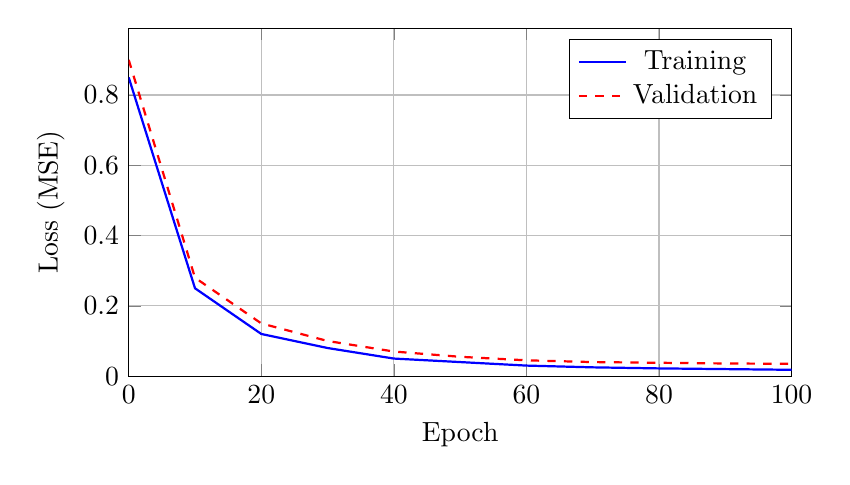
\begin{tikzpicture}
\begin{axis}[
    width=10cm,
    height=6cm,
    xlabel={Epoch},
    ylabel={Loss (MSE)},
    legend pos=north east,
    grid=major,
    xmin=0, xmax=100,
    ymin=0
]
\addplot[thick, blue] coordinates {
    (0, 0.85) (10, 0.25) (20, 0.12) (30, 0.08) (40, 0.05)
    (50, 0.04) (60, 0.03) (70, 0.025) (80, 0.022) (90, 0.02) (100, 0.018)
};
\addplot[thick, red, dashed] coordinates {
    (0, 0.90) (10, 0.28) (20, 0.15) (30, 0.10) (40, 0.07)
    (50, 0.055) (60, 0.045) (70, 0.04) (80, 0.038) (90, 0.036) (100, 0.035)
};
\legend{Training, Validation}
\end{axis}
\end{tikzpicture}
\caption{Training loss curve for neural network motor controller. The gap between training and validation loss indicates slight overfitting.}
\label{fig:training_loss}
\end{figure}

\subsection{Phase 3: Export and Deployment}

\subsubsection{Convert to C Code}

For deployment on Arduino, convert the trained weights to arrays suitable for embedded systems.

\begin{algorithm}[htbp]
\caption{Export Weights for Embedded Deployment}
\label{alg:export_weights}
\begin{algorithmic}[1]
\State \textbf{Input:} Trained model with parameters $\theta$, normalization constants $\mu_u$, $\sigma_u$
\State \textbf{Output:} Header file with weight arrays
\State
\Function{ExportWeights}{model, filename}
    \State Open file for writing
    \For{each parameter $(\text{name}, \mathbf{W})$ in model}
        \State $\mathbf{w}_{\text{flat}} \gets \text{Flatten}(\mathbf{W})$
        \State Write array declaration: ``const float name[] = \{$w_1, w_2, \ldots$\}''
    \EndFor
    \State Write: ``const float control\_mean = $\mu_u$''
    \State Write: ``const float control\_std = $\sigma_u$''
    \State Close file
\EndFunction
\end{algorithmic}
\end{algorithm}

\subsubsection{Arduino Neural Network Implementation}

\begin{algorithm}[htbp]
\caption{Neural Network Inference on Microcontroller}
\label{alg:nn_inference}
\begin{algorithmic}[1]
\State \textbf{Constants:} $n_{\text{in}} = 3$, $n_h = 32$, weight arrays from exported file
\State \textbf{Buffers:} $\mathbf{h}_1[n_h]$, $\mathbf{h}_2[n_h]$
\State
\Function{ReLU}{$x$}
    \If{$x > 0$}
        \State \Return $x$
    \Else
        \State \Return $0$
    \EndIf
\EndFunction
\State
\Function{NeuralNetworkControl}{error, velocity, error\_integral}
    \State \Comment{Normalize inputs using training statistics}
    \State $\mathbf{x}[0] \gets (\text{error} - \mu_e) / \sigma_e$
    \State $\mathbf{x}[1] \gets (\text{velocity} - \mu_v) / \sigma_v$
    \State $\mathbf{x}[2] \gets (\text{error\_integral} - \mu_{\int e}) / \sigma_{\int e}$
    \State
    \State \Comment{Layer 1: input to hidden1}
    \For{$i = 0$ to $n_h - 1$}
        \State $h_1[i] \gets b_1[i] + \sum_{j=0}^{n_{\text{in}}-1} W_1[i, j] \cdot x[j]$
        \State $h_1[i] \gets \text{ReLU}(h_1[i])$
    \EndFor
    \State
    \State \Comment{Layer 2: hidden1 to hidden2}
    \For{$i = 0$ to $n_h - 1$}
        \State $h_2[i] \gets b_2[i] + \sum_{j=0}^{n_h-1} W_2[i, j] \cdot h_1[j]$
        \State $h_2[i] \gets \text{ReLU}(h_2[i])$
    \EndFor
    \State
    \State \Comment{Layer 3: hidden2 to output}
    \State $\text{output} \gets b_3 + \sum_{j=0}^{n_h-1} W_3[j] \cdot h_2[j]$
    \State
    \State \Comment{Denormalize output}
    \State $\text{output} \gets \text{output} \cdot \sigma_u + \mu_u$
    \State \Return $\text{Clamp}(\text{output}, -255, 255)$
\EndFunction
\end{algorithmic}
\end{algorithm}

\subsection{Phase 4: Evaluation and Comparison}

Run both controllers on identical reference trajectories and compare performance.

\begin{figure}[htbp]
\centering
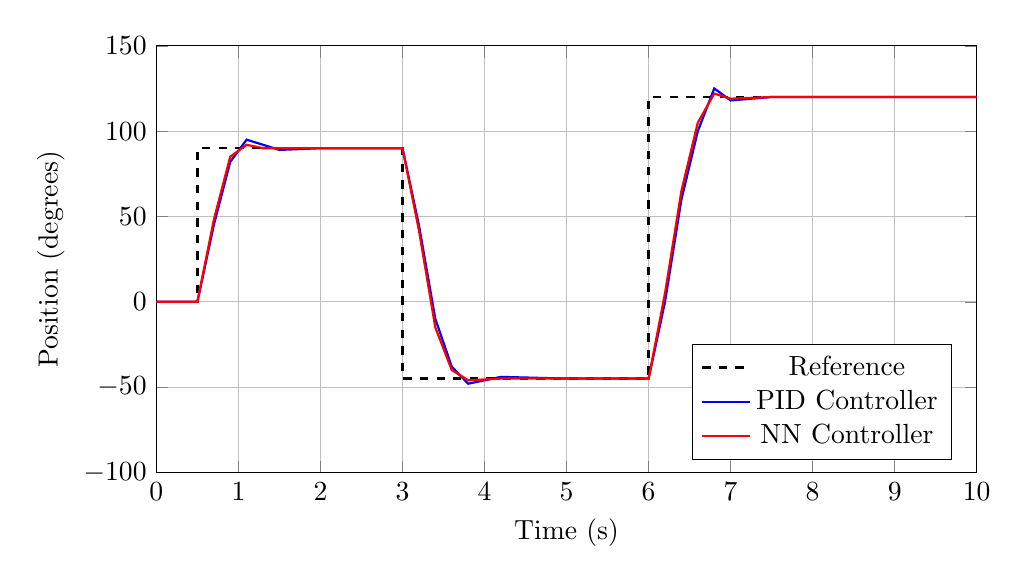
\begin{tikzpicture}
\begin{axis}[
    width=12cm,
    height=7cm,
    xlabel={Time (s)},
    ylabel={Position (degrees)},
    legend pos=south east,
    grid=major,
    xmin=0, xmax=10,
    ymin=-100, ymax=150
]
% Reference
\addplot[thick, black, dashed] coordinates {
    (0, 0) (0.5, 0) (0.5, 90) (3, 90) (3, -45) (6, -45) (6, 120) (10, 120)
};

% PID response
\addplot[thick, blue] coordinates {
    (0, 0) (0.5, 0) (0.7, 45) (0.9, 82) (1.1, 95) (1.3, 92) (1.5, 89)
    (2, 90) (3, 90) (3.2, 45) (3.4, -10) (3.6, -38) (3.8, -48)
    (4.2, -44) (5, -45) (6, -45) (6.2, 0) (6.4, 60) (6.6, 100)
    (6.8, 125) (7.0, 118) (7.5, 120) (10, 120)
};

% NN response
\addplot[thick, red] coordinates {
    (0, 0) (0.5, 0) (0.7, 48) (0.9, 85) (1.1, 92) (1.3, 90) (1.5, 90)
    (2, 90) (3, 90) (3.2, 42) (3.4, -15) (3.6, -40) (3.8, -46)
    (4.2, -45) (5, -45) (6, -45) (6.2, 5) (6.4, 65) (6.6, 105)
    (6.8, 122) (7.0, 119) (7.5, 120) (10, 120)
};

\legend{Reference, PID Controller, NN Controller}
\end{axis}
\end{tikzpicture}
\caption{Comparison of PID and neural network controller responses to step reference changes. The NN controller (trained via behavioral cloning) closely matches the PID response.}
\label{fig:pid_vs_nn}
\end{figure}

\subsubsection{Quantitative Metrics}

Compute performance metrics over the test trajectory:

\begin{table}[htbp]
\centering
\caption{Performance Comparison: PID vs Neural Network Controller}
\label{tab:performance}
\begin{tabular}{lcc}
\toprule
\textbf{Metric} & \textbf{PID} & \textbf{Neural Network} \\
\midrule
RMS Tracking Error (deg) & 5.2 & 5.8 \\
Maximum Overshoot (\%) & 8.3 & 6.1 \\
Settling Time (s) & 0.85 & 0.78 \\
Control Effort (RMS) & 112 & 108 \\
Computation Time ($\mu$s) & 15 & 180 \\
\bottomrule
\end{tabular}
\end{table}

\subsection{Discussion}

The experiment demonstrates several key points. First, behavioral cloning works: the neural network successfully learned to imitate the PID controller without explicit knowledge of PID theory. Second, performance is comparable, with tracking error similar between controllers and the NN showing slightly less overshoot in step responses. Third, while the NN requires more computation per control cycle (180 $\mu$s vs 15 $\mu$s), it remains feasible at 50 Hz on the Arduino Mega. Finally, the NN inherits the limitations of its teacher and cannot exceed PID performance without additional training techniques.

Extensions to this experiment include training on optimal trajectories from MPC rather than suboptimal PID data, online fine-tuning using reinforcement learning to improve beyond the teacher's performance, and incorporating disturbance rejection capabilities through data augmentation or adversarial training.


\section{Worked Examples}

\begin{examplebox}[Computing the Output of a Two-Layer Network]
\textbf{Problem:} Consider a neural network with input $\mathbf{x} = [1, 2]^T$, a hidden layer with 2 neurons having weights $\mathbf{W}^{(1)} = \begin{bmatrix} 0.5 & -0.3 \\ 0.2 & 0.8 \end{bmatrix}$ and biases $\mathbf{b}^{(1)} = \begin{bmatrix} 0.1 \\ -0.2 \end{bmatrix}$, and an output layer with 1 neuron having weights $\mathbf{W}^{(2)} = \begin{bmatrix} 0.7 & 0.4 \end{bmatrix}$ and bias $b^{(2)} = 0.3$. The activation function is ReLU for the hidden layer and linear for the output. Compute the network output.

\textbf{Solution:}

\textbf{Step 1: Hidden layer pre-activation}
\begin{align}
\mathbf{z}^{(1)} &= \mathbf{W}^{(1)}\mathbf{x} + \mathbf{b}^{(1)} \\
&= \begin{bmatrix} 0.5 & -0.3 \\ 0.2 & 0.8 \end{bmatrix} \begin{bmatrix} 1 \\ 2 \end{bmatrix} + \begin{bmatrix} 0.1 \\ -0.2 \end{bmatrix} \\
&= \begin{bmatrix} 0.5(1) + (-0.3)(2) \\ 0.2(1) + 0.8(2) \end{bmatrix} + \begin{bmatrix} 0.1 \\ -0.2 \end{bmatrix} \\
&= \begin{bmatrix} -0.1 \\ 1.8 \end{bmatrix} + \begin{bmatrix} 0.1 \\ -0.2 \end{bmatrix} = \begin{bmatrix} 0 \\ 1.6 \end{bmatrix}
\end{align}

\textbf{Step 2: Hidden layer activation (ReLU)}
\begin{equation}
\mathbf{h}^{(1)} = \text{ReLU}(\mathbf{z}^{(1)}) = \begin{bmatrix} \max(0, 0) \\ \max(0, 1.6) \end{bmatrix} = \begin{bmatrix} 0 \\ 1.6 \end{bmatrix}
\end{equation}

\textbf{Step 3: Output layer}
\begin{align}
y &= \mathbf{W}^{(2)}\mathbf{h}^{(1)} + b^{(2)} \\
&= \begin{bmatrix} 0.7 & 0.4 \end{bmatrix} \begin{bmatrix} 0 \\ 1.6 \end{bmatrix} + 0.3 \\
&= 0.7(0) + 0.4(1.6) + 0.3 = 0.64 + 0.3 = \boxed{0.94}
\end{align}
\end{examplebox}

\begin{examplebox}[Backpropagation by Hand]

\textbf{Problem:} For the network in Example 1, compute the gradient $\partial \mathcal{L}/\partial \mathbf{W}^{(1)}$ if the target is $y^* = 0.5$ and we use MSE loss.

\textbf{Solution:}

\textbf{Step 1: Compute loss}
\begin{equation}
\mathcal{L} = \frac{1}{2}(y - y^*)^2 = \frac{1}{2}(0.94 - 0.5)^2 = \frac{1}{2}(0.44)^2 = 0.0968
\end{equation}

\textbf{Step 2: Output layer gradient}
\begin{equation}
\frac{\partial \mathcal{L}}{\partial y} = y - y^* = 0.94 - 0.5 = 0.44
\end{equation}

\textbf{Step 3: Backpropagate to hidden layer}
\begin{equation}
\frac{\partial \mathcal{L}}{\partial \mathbf{h}^{(1)}} = \left(\mathbf{W}^{(2)}\right)^T \frac{\partial \mathcal{L}}{\partial y} = \begin{bmatrix} 0.7 \\ 0.4 \end{bmatrix} \cdot 0.44 = \begin{bmatrix} 0.308 \\ 0.176 \end{bmatrix}
\end{equation}

\textbf{Step 4: Backpropagate through ReLU}

The ReLU derivative is 1 where input $> 0$ and 0 otherwise:
\begin{equation}
\frac{\partial \mathbf{h}^{(1)}}{\partial \mathbf{z}^{(1)}} = \begin{bmatrix} 0 & 0 \\ 0 & 1 \end{bmatrix}
\end{equation}
(diagonal matrix where $z_1 = 0 \leq 0$ and $z_2 = 1.6 > 0$)

\begin{equation}
\frac{\partial \mathcal{L}}{\partial \mathbf{z}^{(1)}} = \frac{\partial \mathbf{h}^{(1)}}{\partial \mathbf{z}^{(1)}} \cdot \frac{\partial \mathcal{L}}{\partial \mathbf{h}^{(1)}} = \begin{bmatrix} 0 \\ 0.176 \end{bmatrix}
\end{equation}

\textbf{Step 5: Gradient with respect to $\mathbf{W}^{(1)}$}
\begin{align}
\frac{\partial \mathcal{L}}{\partial \mathbf{W}^{(1)}} &= \frac{\partial \mathcal{L}}{\partial \mathbf{z}^{(1)}} \mathbf{x}^T \\
&= \begin{bmatrix} 0 \\ 0.176 \end{bmatrix} \begin{bmatrix} 1 & 2 \end{bmatrix} \\
&= \boxed{\begin{bmatrix} 0 & 0 \\ 0.176 & 0.352 \end{bmatrix}}
\end{align}

Note that the first row has zero gradient because the first neuron's ReLU was inactive (``dead'').
\end{examplebox}

\subsection{Example 3: Designing NN Architecture for Control}

\textbf{Problem:} Design a neural network controller for a quadrotor attitude control problem. The state is $\mathbf{x} = [\phi, \theta, \psi, p, q, r]^T$ (roll, pitch, yaw angles and angular rates). The output is $\mathbf{u} = [\tau_\phi, \tau_\theta, \tau_\psi]^T$ (torques). Specify architecture and justify choices.

\textbf{Solution:}

\textbf{Input layer:} 6 neurons (one per state variable)

Alternatively, include error terms if tracking a reference:
$\mathbf{x}_{\text{input}} = [\phi - \phi_r, \theta - \theta_r, \psi - \psi_r, p, q, r]^T$ (still 6 inputs)

\textbf{Hidden layers:} Two hidden layers with 64 neurons each.

This architecture is justified as follows. Two layers provide sufficient depth for nonlinear function approximation while remaining tractable for training. The choice of 64 neurons per layer is common for moderate-complexity control problems, representing roughly 10$\times$ the input dimension. The total number of parameters is $(6 \times 64 + 64) + (64 \times 64 + 64) + (64 \times 3 + 3) = 4,867$, which is small enough to train efficiently yet large enough to capture the required nonlinearities.

For activation functions, the hidden layers use ReLU due to its computational efficiency and ability to avoid vanishing gradients during training. The output layer uses tanh scaled by the maximum torque $\tau_{\max}$ to naturally bound the control outputs within physically realizable limits.

The output layer uses tanh to naturally bound outputs:
\begin{equation}
\mathbf{u} = \tau_{\max} \cdot \tanh(\mathbf{W}^{(L)}\mathbf{h}^{(L-1)} + \mathbf{b}^{(L)})
\end{equation}

\textbf{Architecture summary:}
\begin{equation}
\boxed{\text{Input}(6) \to \text{Dense}(64, \text{ReLU}) \to \text{Dense}(64, \text{ReLU}) \to \text{Dense}(3, \text{tanh})}
\end{equation}

\hrulefill

\subsection{Example 4: Training NN to Approximate a Known Function}

\textbf{Problem:} Train a neural network to approximate the nonlinear function $f(x) = \sin(x) + 0.5\sin(3x)$ on $[-\pi, \pi]$.

\textbf{Solution:}

\begin{algorithm}[htbp]
\caption{Training Neural Network to Approximate Nonlinear Function}
\label{alg:function_approximation}
\begin{algorithmic}[1]
\State \textbf{Target function:} $f(x) = \sin(x) + 0.5\sin(3x)$ on $[-\pi, \pi]$
\State
\State \Comment{Generate training data}
\State $\mathbf{x}_{\text{train}} \gets \text{LinSpace}(-\pi, \pi, 200)$
\State $\mathbf{y}_{\text{train}} \gets \sin(\mathbf{x}_{\text{train}}) + 0.5 \sin(3 \mathbf{x}_{\text{train}})$
\State
\State \Comment{Define network: $1 \to 32 \to 32 \to 1$ with tanh activations}
\State Initialize network parameters $\theta$
\State Set learning rate $\eta \gets 0.01$
\State
\For{$\text{epoch} = 1$ to $1000$}
    \State $\hat{\mathbf{y}} \gets \text{Forward}(\mathbf{x}_{\text{train}}; \theta)$
    \State $\mathcal{L} \gets \text{MSE}(\hat{\mathbf{y}}, \mathbf{y}_{\text{train}})$
    \State $\nabla_\theta \mathcal{L} \gets \text{Backpropagation}(\mathcal{L})$
    \State $\theta \gets \theta - \eta \cdot \text{AdamUpdate}(\nabla_\theta \mathcal{L})$
\EndFor
\State
\State \Comment{Expected convergence: Loss $\approx 5.6 \times 10^{-5}$ after 1000 epochs}
\end{algorithmic}
\end{algorithm}

After 1000 epochs, the network achieves MSE $\approx 5.6 \times 10^{-5}$, demonstrating successful approximation of the nonlinear target function.

\hrulefill

\subsection{Example 5: Analyzing NN Controller vs Linear Controller}

\textbf{Problem:} Compare a neural network controller with a linear state feedback controller $u = -\mathbf{K}\mathbf{x}$ for a nonlinear pendulum system near the upright equilibrium. Discuss when each is preferred.

\textbf{Solution:}

The inverted pendulum dynamics are:
\begin{equation}
\ddot{\theta} = \frac{g}{\ell}\sin\theta - \frac{b}{m\ell^2}\dot{\theta} + \frac{1}{m\ell^2}u
\end{equation}

\textbf{Linear controller (LQR):} The approach linearizes about $\theta = 0$ using the approximation $\sin\theta \approx \theta$, designs an LQR gain $\mathbf{K} = [K_\theta, K_{\dot{\theta}}]$, and implements the control law $u = -K_\theta\theta - K_{\dot{\theta}}\dot{\theta}$.

The linear controller offers several advantages: stability is guaranteed provided the linearization remains valid, the gains are interpretable and can be tuned systematically, the controller is optimal for the linearized system, and no training data is required. However, limitations include performance degradation for large $\theta$ where the linearization breaks down, and the inability to handle constraints directly in the control law.

\textbf{Neural network controller:} The approach trains a mapping $u = f_\theta(\theta, \dot{\theta})$ using data from near-optimal trajectories, learning the control law directly from examples.

The neural network controller offers complementary advantages: it can learn a nonlinear control law valid for large angles far from the equilibrium, can implicitly learn constraint satisfaction through training data that respects constraints, and can incorporate more complex objectives beyond quadratic costs. The limitations include no stability guarantee without additional analysis, the requirement for training data collection, and black-box behavior that makes debugging and certification difficult.

\textbf{Comparison experiment:}

\begin{table}[htbp]
\centering
\caption{Performance Comparison for Pendulum Swing-Up}
\label{tab:pendulum_comparison}
\begin{tabular}{lcc}
\toprule
\textbf{Initial Angle} & \textbf{LQR Success} & \textbf{NN Success} \\
\midrule
$\pm 10^\circ$ & Yes & Yes \\
$\pm 30^\circ$ & Yes & Yes \\
$\pm 60^\circ$ & Marginal & Yes \\
$\pm 90^\circ$ & No & Yes \\
$\pm 150^\circ$ (swing-up) & No & Yes \\
\bottomrule
\end{tabular}
\end{table}

\textbf{Conclusion:} Use linear control when operating near equilibrium with stability guarantees needed. Use NN control for large operating regions or when linear approximations are inadequate.

\hrulefill

\subsection{Example 6: Neural Network for System Identification}

\textbf{Problem:} A black-box system has unknown dynamics. Given input-output data, design and train a neural network model.

\textbf{Given data:} 1000 samples of $(\mathbf{x}[k], u[k], \mathbf{x}[k+1])$ where $\mathbf{x} = [x_1, x_2]^T$.

\textbf{Solution:}

\textbf{Step 1: Architecture design}

Model: $\hat{\mathbf{x}}[k+1] = f_\theta(\mathbf{x}[k], u[k])$

Input dimension: 3 (two states + one control)

Output dimension: 2 (two states)

Architecture: $3 \to 64 \to 64 \to 2$ with ReLU activations.

\textbf{Step 2: Training}

\begin{algorithm}[htbp]
\caption{System Identification Training}
\label{alg:sysid_training}
\begin{algorithmic}[1]
\State \textbf{Input:} Data $\{(\mathbf{x}[k], u[k], \mathbf{x}[k+1])\}_{k=1}^{N}$
\State \textbf{Network:} $3 \to 64 \to 64 \to 2$ with ReLU activations
\State
\State Construct input matrix $\mathbf{X}_{\text{current}}$ with rows $[\mathbf{x}[k]^T, u[k]]$
\State Construct target matrix $\mathbf{X}_{\text{next}}$ with rows $\mathbf{x}[k+1]^T$
\State Initialize network parameters $\theta$
\State Set learning rate $\eta \gets 0.001$
\State
\For{$\text{epoch} = 1$ to $500$}
    \State $\hat{\mathbf{X}}_{\text{next}} \gets \text{Forward}(\mathbf{X}_{\text{current}}; \theta)$
    \State $\mathcal{L} \gets \text{MSE}(\hat{\mathbf{X}}_{\text{next}}, \mathbf{X}_{\text{next}})$
    \State $\nabla_\theta \mathcal{L} \gets \text{Backpropagation}(\mathcal{L})$
    \State $\theta \gets \theta - \eta \cdot \text{AdamUpdate}(\nabla_\theta \mathcal{L})$
\EndFor
\end{algorithmic}
\end{algorithm}

\textbf{Step 3: Validation}

Test multi-step prediction accuracy:
\begin{equation}
\text{Multi-step error} = \frac{1}{T}\sum_{k=0}^{T} \|\mathbf{x}[k] - \hat{\mathbf{x}}[k]\|
\end{equation}
where $\hat{\mathbf{x}}$ is rolled out using the learned model.

If multi-step error grows rapidly, the model may need more training data to cover a wider range of operating conditions, a deeper or wider architecture to capture more complex dynamics, or a recurrent structure such as LSTM or GRU layers to capture longer-term dependencies in the system behavior.


\section{Chapter Summary}

This chapter introduced neural networks as powerful tools for control system design, capable of learning complex nonlinear mappings from data. Key concepts include the following.

The \textbf{historical development} of neural networks for control spans from McCulloch-Pitts neurons (1943) through the Perceptron (1958), backpropagation (1974/1986), and the landmark work of Narendra and Parthasarathy (1990) applying neural networks to control. Understanding this history illuminates both the capabilities and limitations of modern approaches.

The \textbf{neural network fundamentals} begin with the artificial neuron, which computes $y = \sigma(\mathbf{w}^T\mathbf{x} + b)$. Multi-layer networks achieve universal function approximation through composition of these simple nonlinear functions, providing the theoretical foundation for their use in control.

When used as a \textbf{controller}, neural networks directly map states to control actions via $\mathbf{u} = f_\theta(\mathbf{x})$. Training proceeds through behavioral cloning (supervised learning from expert data) or reinforcement learning for cases where optimal demonstrations are unavailable.

When used as a \textbf{plant model}, neural networks learn dynamics $\hat{\mathbf{x}}[k+1] = f_\theta(\mathbf{x}[k], \mathbf{u}[k])$ for use in simulation or model predictive control, enabling control design when first-principles models are unavailable.

The \textbf{training} process relies on backpropagation to compute gradients efficiently. Backpropagation through time handles sequential dynamics inherent in control problems. Modern optimizers like Adam improve convergence and reduce sensitivity to learning rate selection.

Key \textbf{challenges} remain: neural network controllers lack inherent stability guarantees, require significant training data that may be expensive to collect, and may not transfer well from simulation to reality due to the sim-to-real gap.

Finally, \textbf{hybrid approaches} that combine neural networks with physics-based models through residual learning or physics-informed neural networks leverage the strengths of both data-driven and first-principles methods.


\newpage
\section{Exercises}

\begin{exercise}
A neural network has architecture $2 \to 3 \to 1$ with sigmoid activations. If $\mathbf{W}^{(1)} = \begin{bmatrix} 1 & 0 \\ 0 & 1 \\ 1 & 1 \end{bmatrix}$, $\mathbf{b}^{(1)} = \mathbf{0}$, $\mathbf{W}^{(2)} = [1, 1, -2]$, $b^{(2)} = 0$:
(a) Compute the output for input $\mathbf{x} = [0, 0]^T$.
(b) Show that this network approximates the XOR function for inputs in $\{0, 1\}^2$.
(c) Explain why a single-layer network cannot compute XOR.
\end{exercise}

\begin{exercise}
Derive the backpropagation equations for a network with one hidden layer using tanh activation:
(a) Express $\partial \mathcal{L}/\partial \mathbf{W}^{(1)}$ in terms of $\boldsymbol{\delta}^{(2)}$, $\mathbf{W}^{(2)}$, $\mathbf{h}^{(1)}$, and $\mathbf{x}$.
(b) Verify that when $\mathbf{h}^{(1)} \approx \pm 1$ (saturation), gradients vanish.
\end{exercise}

\begin{exercise}
For a DC motor position control problem, design a neural network architecture:
(a) Specify inputs if the goal is to track a reference position $\theta_r$.
(b) Propose a network architecture (layers, widths, activations).
(c) Estimate the total number of parameters.
(d) Describe how you would collect training data.
\end{exercise}

\begin{exercise}
Compare training a neural network controller using:
(a) Behavioral cloning from PID controller data
(b) Direct optimization of tracking error (end-to-end training)
Discuss the advantages and disadvantages of each approach.
\end{exercise}

\begin{exercise}
A neural network model $\hat{\mathbf{x}}[k+1] = f_\theta(\mathbf{x}[k], \mathbf{u}[k])$ is trained with one-step prediction loss. When used for multi-step simulation, prediction errors accumulate.
(a) Explain why errors accumulate.
(b) Propose a modified training procedure to improve multi-step accuracy.
(c) How does this relate to the ``compounding errors'' problem in behavioral cloning?
\end{exercise}

\begin{exercise}
Implement (in Python or MATLAB) a neural network to learn the dynamics of a simple pendulum from simulated data:
(a) Generate 10,000 samples of $(\theta, \dot{\theta}, \tau, \theta_{\text{next}}, \dot{\theta}_{\text{next}})$.
(b) Train a network with architecture $3 \to 32 \to 32 \to 2$.
(c) Evaluate one-step and 100-step prediction accuracy.
(d) Compare with a linear model fit to the same data.
\end{exercise}

\begin{exercise}
Consider a hybrid controller: $u = u_{\text{PID}} + u_{\text{NN}}$ where $u_{\text{PID}} = K_p e + K_d \dot{e}$ and $u_{\text{NN}} = f_\theta(\mathbf{x})$.
(a) What advantages does this structure offer over a pure NN controller?
(b) How would you train $f_\theta$ while keeping PID gains fixed?
(c) Can you provide stability guarantees if the NN output is bounded?
\end{exercise}

\begin{exercise}
The Universal Approximation Theorem guarantees that a neural network can approximate any continuous function. Why doesn't this guarantee that gradient descent will find good weights? Discuss:
(a) Local minima and saddle points
(b) The role of network architecture (depth vs. width)
(c) Implicit regularization from optimization algorithms
\end{exercise}

\begin{exercise}
A neural network controller is trained to stabilize an inverted pendulum using behavioral cloning from an expert (MPC controller). The expert achieves a success rate of 95\% from random initial conditions. After training, the neural network achieves only 70\% success rate. (a) Explain why this performance gap might occur. (b) Propose two different strategies to close this gap. (c) Which strategy would you recommend if safety during training is a primary concern?
\end{exercise}

\begin{exercise}
Consider the problem of learning a dynamics model $\hat{f}$ for use in Model Predictive Control. You have two options: (A) a neural network with 3 hidden layers of 64 neurons each, or (B) a neural network with 1 hidden layer of 256 neurons. Both have approximately the same number of parameters. (a) Discuss the trade-offs between these architectures for dynamics modeling. (b) Which would you expect to generalize better to states outside the training distribution? (c) How would computational cost differ during MPC optimization?
\end{exercise}


\section{Further Reading}

For the foundational treatment of neural networks in control, see Narendra, K.S. and Parthasarathy, K., ``Identification and Control of Dynamical Systems Using Neural Networks,'' \textit{IEEE Transactions on Neural Networks}, vol. 1, no. 1, pp. 4--27, 1990.

For comprehensive coverage of modern deep learning theory and practice, consult Goodfellow, I., Bengio, Y., and Courville, A., \textit{Deep Learning}, MIT Press, 2016.

An excellent integration of machine learning with control systems is provided by Brunton, S.L. and Kutz, J.N., \textit{Data-Driven Science and Engineering: Machine Learning, Dynamical Systems, and Control}, Cambridge University Press, 2019.

The standard reference for reinforcement learning, which extends behavioral cloning to online learning, is Sutton, R.S. and Barto, A.G., \textit{Reinforcement Learning: An Introduction}, 2nd ed., MIT Press, 2018.

For a review of system identification including neural network approaches, see Ljung, L., ``Perspectives on System Identification,'' \textit{Annual Reviews in Control}, vol. 34, no. 1, pp. 1--12, 2010.

The original universal approximation theorem is presented in Cybenko, G., ``Approximation by Superpositions of a Sigmoidal Function,'' \textit{Mathematics of Control, Signals, and Systems}, vol. 2, pp. 303--314, 1989.

\end{chapter}
